\documentclass[12pt,a4paper]{article}
\usepackage{algorithm, algpseudocode, amsmath, amssymb, amsthm, bm, csquotes, emf, empheq, geometry, graphicx, hyperref, listings, mhchem, multirow, siunitx, slashbox, subcaption, upgreek}
\usepackage[italicdiff]{physics}
%\usepackage[section]{placeins}
\usepackage[justification=centering]{caption}
\usepackage[column=O]{cellspace}
\usepackage[extrafootnotefeatures]{xepersian}
\hypersetup{colorlinks=true, urlcolor=cyan}

\title{قطبی کردن تلسکوپ}
\author{آرتین خانعلی، سپهر سلمانی یگانه، صالح شاملو احمدی\\\\
	آزمایشگاه نجوم، ترم تابستان ۱۴۰۲\\دانشکده فیزیک دانشگاه صنعتی شریف}
\date{۲۰ تیر ۱۴۰۲}

\settextfont{Yas}
\ExplSyntaxOn
\cs_set_eq:NN
\etex_iffontchar:D
\tex_iffontchar:D
\cs_undefine:N \c_one
\int_const:Nn \c_one { 1 } 
\ExplSyntaxOff
\setdigitfont{Yas}
\linespread{1.2}

\makeatletter
\g@addto@macro\bfseries{\boldmath}
\makeatother

\setlength\cellspacetoplimit{5pt}
\setlength\cellspacebottomlimit{3pt}
\newcommand{\multlinecell}[1]{\begin{tabular}[c]{@{}c@{}}#1\end{tabular}}

\newcommand{\qfrac}[2]{\left(\frac{#1}{#2}\right)}
\newcommand{\fsqrt}[2]{\sqrt{\frac{#1}{#2}}}
\newcommand{\ddfrac}[2]{{\displaystyle\frac{\displaystyle #1}{\displaystyle #2}}}
\newcommand{\pdvc}[3]{\qfrac{\partial #1}{\partial #2}_{#3}}
\newcommand{\dbar}{{d\mkern-7mu\mathchar'26\mkern-2mu}}
\newcommand*{\defeq}{\mathrel{\vcenter{\baselineskip0.5ex \lineskiplimit0pt
			\hbox{\scriptsize.}\hbox{\scriptsize.}}}
	=}

\newtheorem{theorem}{قضیه}
\newtheorem{lemma}{لم}
\renewcommand\qedsymbol{$\blacksquare$}

\begin{document}
	\maketitle
	\twocolumnfootnotes
	\section{مقدمه}
	در این گزارش، مراحل کلی اولین آزمایش عملی که با تلسکوپ انجام دادیم را بررسی می‌کنیم. هدف کلی، آشنایی با
	قطبی کردن تلسکوپ بوده که برای عکس‌برداری نجومی ضروری است و در تمام رصدهای بعدی قبل از داده‌گیری انجام می‌شود.
	\section{ابزار استفاده شده}
	تلسکوپ شش اینچی نیوتنی \lr{Skywatcher} با مقر استوایی \lr{NEQ3}.
	\section{آماده‌سازی اولیه}
	ابتدا هر تلسکوپ را متناسب با پایه و ابزار مربوط به آن می‌بندیم. در مرحله بعد با جابه‌جایی وزنه‌ها و خود تلسکوپ،
	تعادل آن را روی دو محور تنظیم می‌کنیم. سپس با استفاده از تراز مکانیکی و با تنظیم طول سه پایه‌ی روی زمین تلسکوپ،
	آن را نسبت به سطح کره زمین تراز می‌کنیم (سطوح مخلف، شیب و ناهمواری متفاوت دارند). در مرحله بعد
	چشمی\footnote{\lr{eyepiece}} را با یابنده\footnote{\lr{finder}} همخط می‌کنیم؛ یعنی جایی که یابنده نشان می‌دهد را با
	جایی که چشمی نشان می‌دهد یکی می‌کنیم. در آخر اگر آینه‌های تلسکوپ موازی نبودند (اگر تصویر خارج از فکوس باشد، منابع
	نور نقطه‌ای، مثل ستاره‌ها، باید به شکل قرصی یکنواخت دیده شوند) پیچ‌های مربوط به آن‌ها را تنظیم می‌کنیم.
	
	همخط کردن بدین شکل است که ابتدا با استفاده از یابنده، یک جسم نقطه‌ای نسبت به دید تلسکوپ را پیدا می‌کنیم و در مرکز آن
	قرار می‌دهیم. سپس آن جسم را در وسط چشمی قرار می‌دهیم. در آخر با تنظیم پیچ‌های یابندی، جسم را در وسط آن قرار می‌دهیم.
	\section{هدف از قطبی کردن}
	بدیهتاً آسمان زمین ثابت نیست و به دلیل گردش زمین به دور خود، ستاره‌ها همواره در حال حرکت به سمت غرب هستند. برای
	نورگیری در مدت زمان طولانی، نیاز است که دید تلسکوپ از روی ستاره منحرف نشود و در تصویر همواره در نقطه‌ای ثابت قرار
	داشته باشد. ساده‌ترین روش اصلاح تأثیر گردش زمین، این است که تلسکوپ را با محور زمین همراستا کنیم و با استفاده از یک
	موتور که سرعتی برابر با نرخ گردش زمین دارد، تلسکوپ را حول این محور دوران دهیم. این عملیات توسط استقرار
	استوایی\footnote{\lr{equatorial mount}} انجام می‌شود.
	\begin{figure}[h!]
		\centering
		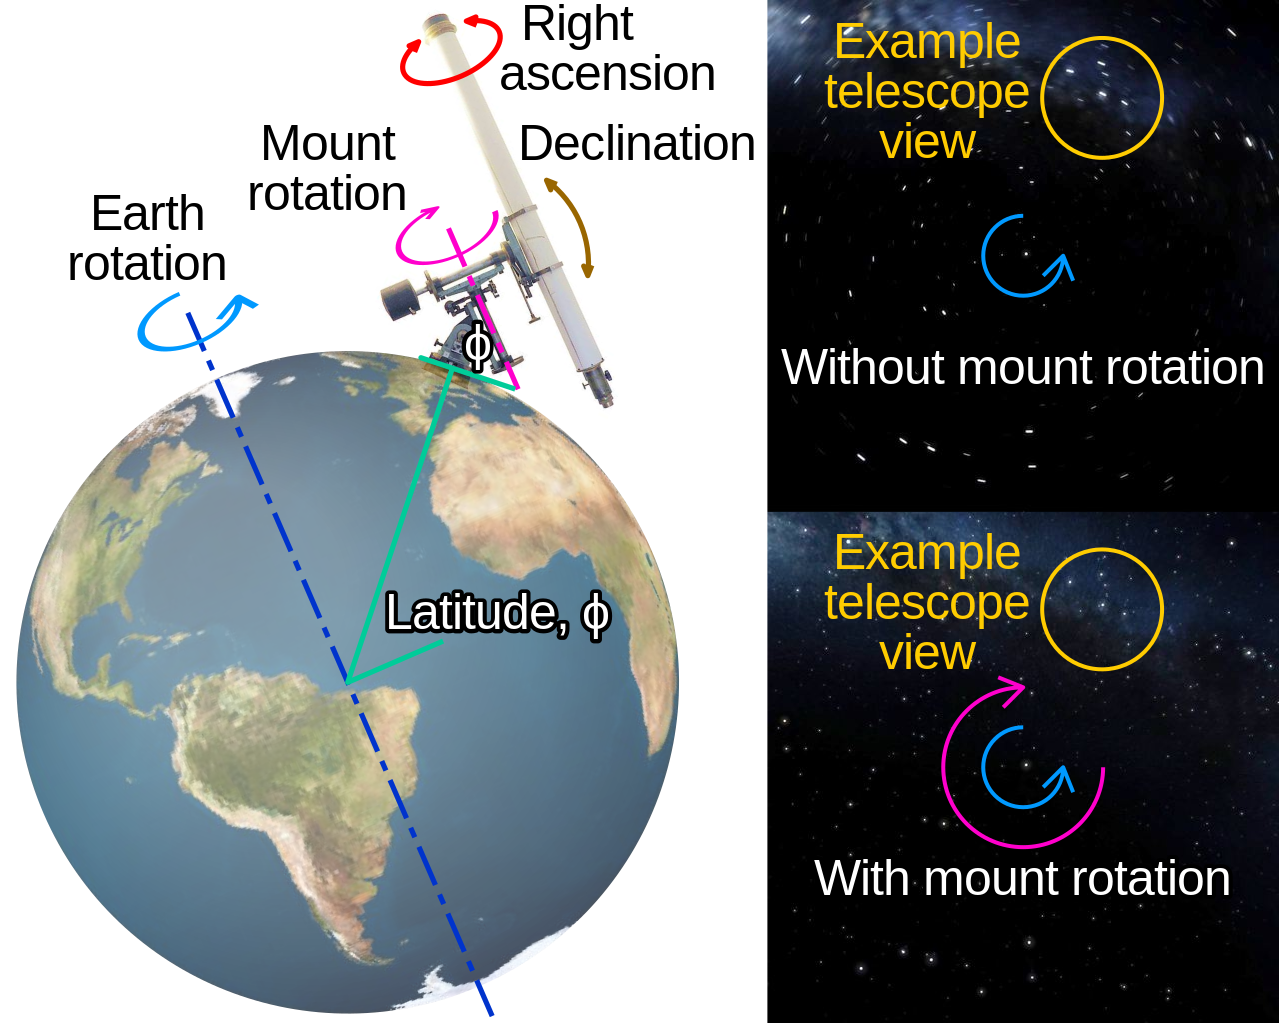
\includegraphics[width=0.9\linewidth]{Equatorial_mount}
		\caption{قطبی کردن و تأثیر آن روی تصویر.\\منبع:
			\href{https://en.wikipedia.org/wiki/File:Equatorial_mount.svg}{کار \lr{cmglee, jimht at shaw dot ca, Rama, Stellarium} در \lr{Wikipedia}}}
	\end{figure}
	\section{فرایند قطبی کردن}
	ابتدا با استفاده از ستاره قطبی\footnote{\lr{Polaris}} تلسکوپ را به صورت حدودی قطبی می‌کنیم؛ در تلسکوپ‌هایی
	که \lr{Polaroscope} دارند، با استفاده از نشانگرش این کار را انجام می‌دهیم. در غیر این صورت، تلسکوپ را روی محور اصلی
	قرار می‌دهیم و با استفاده از پیچ‌های پایه، جهت آن را تنظیم می‌کنیم. معمولاً پیچ‌های فلزی مربوط به تنظیم ارتفاع
	و پیچ‌های پلاستیکی مربوط به سمت هستند. با یک بررسی ساده، واضح است کدام پیچ‌ها مربوط به کدام جهت هستند.
	
	در مرحله بعدی، از روش قطبی کردن انحرافی\footnote{\lr{Drift Alignment}} استفاده می‌کنیم. در این روش ابتدا ستاره‌ای
	را در وسط چشمی قرار می‌دهیم، سپس موتور را روشن می‌کنیم و صبر می‌کنیم تا ستاره در جهت جز جهت شمالی--جنوبی منحرف شود
	(انحراف در جهت غربی--شرقی به دلیل خطای موتور است). سپس با توجه به جهت انحراف، جهت پایه را اصلاح می‌کنیم.
	
	مرحله اول این است که جهت‌های جغرافیایی را روی چشمی تلسکوپ پیدا کنیم. دقت کنید که شرق و غرب آسمان نسبت به شمال و
	جنوب آن برعکس شرق و غرب جغرافیایی هستند؛ یعنی روی چشمی باید ۹۰ درجه ساعتگرد بچرخیم تا روی غرب قرار بگیریم، اما
	وقتی رو به شمال قرار می‌گیریم، غرب جغرافیایی سمت چپ قرار می‌گیرد. برای پیدا کردن غرب، می‌توانیم موتور را خاموش کنیم
	و ببینیم ستارگان به سرعت به چه سمتی حرکت می‌کنند. این جهت، غرب است و از روی آن می‌توانیم بقیه جهات را نیز تعیین کنیم.
	اگر خودمان جهات جغرافیایی را بدانیم، راه دیگر این است که تلسکوپ را از فکوس خارج کنیم و دستمان را از جهتی مشخص وارد
	میدان دید تلسکوپ کنیم. بدین صورت، با اختلالی که در تصویر ایجاد می‌شود، جهت را پیدا می‌کنیم.
	
	به دلیل ثابت بودن عرض جغرافیایی ما در رصدهای مختلف، اگر روی زمین به نسبت صاف قرار گرفته باشیم،
	انحراف ارتفاع تلسکوپ معمولاً کمتر است، پس تنظیم آن را بعد از تنظیم سمت انجام می‌دهیم.
	
	برای تنظیم سمت، ستاره‌ای در نزدیکی تقاطع نصف‌النهار و استوای سماوی  پیدا می‌کنیم. انحراف سمت این ستارگان از بقیه
	سرعت بیشتری دارد و کار را راحت‌تر می‌کند. ما برای این بخش از ستاره \lr{Spica} در نزدیکی ساعت ۹ شب استفاده کردیم. در این
	حالت اگر ستاره به سمت جنوب منحرف شود، محور زیادی رو به شرق است و بالعکس.
	
	برای تنظیم ارتفاع، ستاره‌ای در نزدیکی افق شرقی انتخاب می‌کنیم. چون نزدیک افق آلودگی نوری بیشتر است و جو ضخیم‌تر است،
	احتمالاً مجبور شویم ستاره‌ای حدود ۲۰ درجه بالاتر از افق انتخاب کنیم. ما برای این بخش از ستاره \lr{Altair} در نزدیکی
	ساعت ۳۰:۹ شب استفاده کردیم که البته کمی بالاتر از ۲۰ درجه بود. در این حالت اگر ستاره به سمت جنوب منحرف شود،
	محور زیادی رو به جنوب است و بالعکس.
	
	بعد از تنظیم در هر مرحله، برای تشخیص انحراف حدود دو تا سه دقیقه صبر کردیم. معمولاً انحراف شدید‌تر از این است و در
	حدود ۳۰ ثانیه هم انحراف دیده می‌شود. قبل از گروه ما یک بار تلاش برای قطبی کردن انجام شده بود، به همین دلیل انحراف‌ها
	کمتر بودند.
\end{document}